\documentclass[xcolor=table,aspectratio=169]{beamer}
\usetheme{Madrid}
\usepackage{adjustbox}
\usepackage{dcolumn}
\newcolumntype{d}[1]{D{.}{.}{#1}}
%\usetheme{metropolis}
\usepackage[style=verbose-note, sorting=none, sortcites=true, maxnames=1, giveninits=true, autocite=superscript, doi=false, url=false, isbn=false, backend=biber, citetracker=false, pagetracker=false, bibencoding=utf8, eprint=false]{biblatex}
% \usepackage[backend=bibtex,style=authoryear-comp,citestyle=authoryear-comp,firstinits=true,sorting=none,maxnames=1,doi=false,isbn=false,url=false,eprint=false]{biblatex}
\usepackage[T1]{fontenc}
\usepackage[normalem]{ulem}
\usepackage{pifont}

\definecolor{twitter_blue}{HTML}{1da1f2}
\input{seaborn_colours.tex}

% Gobbling first names

\AtEveryCitekey{%
   \clearfield{shorttitle}%
   \clearfield{month}%
   \clearfield{day}%
   \ifentrytype{article}{%
      \clearfield{title}%
   }{}
   }
\ExecuteBibliographyOptions[online]{eprint=true}

% "blindfootcite" is the equivalent of "footcite" except the number marker does not appear
\newcommand\blfootcite[1]{%
  \begingroup
  \renewcommand\thefootnote{}\footnote{\hspace{-4ex}\cite{#1}}%
  \addtocounter{footnote}{-1}%
  \endgroup
}
\renewcommand*{\multicitedelim}{\textcolor{seaborn_bg_grey_darker}{\addsemicolon}}
\setbeamerfont{footnote}{size=\scriptsize}
\renewcommand\footnoterule{\kern-3pt \color{seaborn_bg_grey_darker}\hrule width \textwidth height 0.4pt \color{black} \kern 2.6pt}

\DeclareSourcemap{
  \maps[datatype=bibtex,overwrite=False]{
   \map{
     \step[fieldsource=journal,
           match={Journal of Chemical Theory and Computation},
           replace={JCTC}]
     \step[fieldsource=journal,
           match={Reviews of Modern Physics},
           replace={Rev. Mod. Phys.}]
     \step[fieldsource=journal,
           match={Reports on Progress in Physics},
           replace={Rep. Prog. Phys.}]
     \step[fieldsource=journal,
           match={Physical Review Letters},
           replace={Phys. Rev. Lett.}]
     \step[fieldsource=journal,
           match={Physical Review},
           replace={Phys. Rev.}]
     \step[fieldsource=journal,
           match={B - Condensed Matter and Materials Physics},
           replace={B}]
     \step[fieldsource=journal,
           match={Journal of Chemical Physics},
           replace={J. Chem. Phys.}]
     \step[fieldsource=journal,
           match={Annual Review of Materials Research},
           replace={Annu. Rev. Mater. Res.}]
   }
  }
}

\renewbibmacro{in:}{}
\DeclareFieldFormat{pages}{\mkfirstpage{#1}}
\beamertemplatenavigationsymbolsempty
\bibliography{references.bib}
\setbeamertemplate{bibliography item}[text]
\renewbibmacro{in:}{}
\AtEveryBibitem{\clearfield{title}}
\AtEveryBibitem{\clearfield{month}}
\AtEveryBibitem{\clearfield{pages}}
\DeclareNameAlias{default}{given-family}

% \renewcommand*{\bibfont}{\tiny}
\usepackage{amssymb}
\usepackage{epsfig}
\usepackage{psfrag}
\usepackage{wrapfig}
\usepackage{graphicx}
\usepackage{color}
\usepackage[table]{xcolor}
\usepackage{amsmath}
\usepackage{multimedia}
\usepackage{subcaption}
%\usepackage{style}
\usepackage{verbatim}
\usepackage{multicol}
\usepackage[table]{xcolor}
\usepackage{tabularx}
\usepackage{cleveref}
% Tikz
\usepackage{tikz}
\usetikzlibrary{positioning,shapes,arrows,backgrounds,fit,calc,external,trees,tikzmark,fadings}
\tikzfading[name=fade bottom,top color=transparent!0, bottom color=transparent!100]
% \tikzexternalize[prefix=tikzfigures/]
\tikzstyle{dummy} = []
\tikzstyle{line} = [draw, thick, -latex']
\tikzstyle{headless_line} = [draw, thick, -]
\tikzstyle{default}    = [rectangle, text centered, rounded corners, text=black, font=\sffamily\footnotesize, align=center]
\tikzstyle{default_text}    = [rectangle, text width=10cm, text=black,anchor=north west, font=\sffamily]
\tikzstyle{boxwhite} = [default, fill=white, rounded corners=0.1cm]
\tikzstyle{cp}    = [default, fill=seaborn_blue, text=white, text width=2.8cm, minimum height=0.5cm]
\tikzstyle{pw}    = [cp, fill=seaborn_green]
\tikzstyle{wannier90}    = [cp, fill=seaborn_cyan]
\tikzstyle{bespoke}    = [cp, fill=seaborn_magenta]
\tikzstyle{observable}    = [cp, fill=seaborn_red]
\tikzset{
  -|-/.style={
    to path={
      (\tikztostart) -| ($(\tikztostart)!#1!(\tikztotarget)$) |- (\tikztotarget)
      \tikztonodes
    }
  },
  -|-/.default=0.5,
  |-|/.style={
    to path={
      (\tikztostart) |- ($(\tikztostart)!#1!(\tikztotarget)$) -| (\tikztotarget)
      \tikztonodes
    }
  },
  |-|/.default=0.5,
}

\newlength{\myyshift}
\setlength{\myyshift}{0.05cm}

\usepackage{lipsum}
\usetikzlibrary{calc}
\newlength{\myfigscale}
\setlength{\myfigscale}{0.3cm}
\usepackage{smartdiagram}
\usesmartdiagramlibrary{additions}
\usepackage{multicol}
\usepackage{helvet}
% \usepackage{sansmathfonts}
% \sansmath
\usepackage{cancel} % for \cancel
\usepackage[normalem]{ulem} % for sout (strike out)
\usepackage{tcolorbox}
\tcbuselibrary{skins,hooks}
\tcbset{colframe=structure,fonttitle=\bfseries,beamer, clip upper, boxsep=0pt, sharp corners=all, no shadow, left skip=0pt, right skip=0pt, coltext=white}

% For electron orbital diagrams
\usepackage{tikzorbital}
% Changing defaults
\pgfkeys{tikzorbital/drawLevel/width = 0.666666}
\pgfkeys{tikzorbital/drawLevel/style = {line width = 1pt, color = black!80, line cap = round}}
\pgfkeys{tikzorbital/drawLevel/spinlength = 0.666666}
\pgfkeys{tikzorbital/drawLevel/spinstyle = {very thick, color = black!80, -stealth}}

\input{seaborn_colours.tex}

% For tikz diagrams with nodes appearing on each slide
\tikzset{
  invisible/.style={opacity=0},
  visible on/.style={alt={#1{}{invisible}}},
  alt/.code args={<#1>#2#3}{%
    \alt<#1>{\pgfkeysalso{#2}}{\pgfkeysalso{#3}} % \pgfkeysalso doesn't change the path
  },
}

\usepackage{array}
\usepackage{multirow}
% \newcolumntype{L}[1]{>{\raggedright\let\newline\\\arraybackslash\hspace{0pt}}m{#1}}
% \newcolumntype{C}[1]{>{\centering\let\newline\\\arraybackslash\hspace{0pt}}m{#1}}
% \newcolumntype{R}[1]{>{\raggedleft\let\newline\\\arraybackslash\hspace{0pt}}m{#1}}
\newcolumntype{L}{>{\raggedright\arraybackslash}X}
\newcolumntype{C}{>{\centering\arraybackslash}X}
\newcolumntype{R}{>{\raggedleft\arraybackslash}X}

\newcommand{\bra}[1]{\langle #1|}
\newcommand{\braket}[2]{\langle #1|#2\rangle}
\newcommand{\braopket}[3]{\langle #1|#2|#3\rangle}
\newcommand{\ket}[1]{|#1\rangle}
\newcommand{\nline}{\nonumber \\}
\newcommand{\Trace}{\mathsf{Tr}}

\renewcommand{\ttdefault}{pcr} % enables bold fixed width font
\numberwithin{equation}{section}
% \usefonttheme{professionalfonts}
%\usefonttheme[stillsansseriflarge,stillsansserifsmall]{serif}
\usepackage{siunitx,booktabs}
% \AtBeginDocument{\sisetup{math-rm=\mathsf, text-rm=\sffamily}}
\AtBeginEnvironment{frame}{\setcounter{footnote}{0}}

\newlength{\myimscale}


% For code blocks in latex
% Taken from https://github.com/daveyarwood/gruvbox-pygments
% N.B.
%  - frame must have [fragile]
%  - use \begin{onlyenv} not \only
%  - after a lot of mucking around, I created gruvbox_plain as another style
%    that exclusively uses gruvbox's bg and fg with no syntax highlighting
%  - use [autogobble] to remove leading indentations

\usepackage{minted}
\usemintedstyle{gruvbox-dark}
\definecolor{gruvbox_dark_bg}{HTML}{282828}
\definecolor{gruvbox_fg}{HTML}{ebdbb2}
\definecolor{kgrey}{HTML}{2b2828}
\setminted[python]{bgcolor=gruvbox_dark_bg}
\setminted[json]{bgcolor=gruvbox_dark_bg}
\setminted[shell-session]{style=gruvbox_plain, bgcolor=gruvbox_dark_bg}

% \lstset{breaklines,breakatwhitespace,breakautoindent=false,showstringspaces=false}
% \lstset{keywordstyle=\color{purple}}
% \lstset{identifierstyle=\color{blue}}
% \lstset{basicstyle=\fontfamily{pcr}\fontsize{9pt}{9pt}\selectfont}
% %\lstset{numbers=left, numberstyle=\tiny, stepnumber=1, numbersep=5pt}
% \lstset{linewidth=4.9in,xleftmargin=10pt}

\setbeamercolor{frametitle}{bg=kgrey,fg=white}
\setbeamerfont{normal text}{family=helvet}
\setbeamerfont{local structure}{family=helvet}

\setbeamercolor*{author in head/foot}{bg=seaborn_blue}
\setbeamercolor*{logo in head/foot}{bg=seaborn_blue,fg=white}
\setbeamercolor*{title in head/foot}{bg=seaborn_blue,fg=kgrey}
\setbeamercolor*{date in head/foot}{bg=seaborn_blue,fg=white}
\setbeamercolor{title}{fg=kgrey}
\setbeamercolor{under headline}{bg=seaborn_red}
\setbeamercolor{footline}{bg=seaborn_blue}
\setbeamercolor{caption name}{fg=seaborn_blue}
\setbeamercolor{block title}{bg=kgrey,fg=white}
\setbeamercolor{block body}{bg=seaborn_bg_grey,fg=black}

% Footnote style and colour
% No line over footnote
\setbeamercolor{footnote}{fg=seaborn_bg_grey_darker}
\setbeamertemplate{enumerate items}[default]
\setbeamertemplate{blocks}[default]
\setbeamertemplate{itemize items}{\normalsize $\bullet$}
\setbeamercolor{description item}{fg=seaborn_blue}
\setbeamercolor{enumerate item}{fg=seaborn_blue}
\setbeamercolor{itemize item}{fg=seaborn_blue}
\setbeamercolor{itemize subitem}{fg=seaborn_blue}
\setbeamercolor{itemize subsubitem}{fg=seaborn_blue}
\setbeamercolor*{bibliography entry title}{fg=seaborn_bg_grey_darker}
\setbeamercolor*{bibliography entry author}{fg=seaborn_bg_grey_darker}
\setbeamercolor*{bibliography entry location}{fg=seaborn_bg_grey_darker}
\setbeamercolor*{bibliography entry note}{fg=seaborn_bg_grey_darker}
% and kill the abominable icon
\setbeamertemplate{bibliography item}[text]

\setbeamerfont*{title in head/foot}{size=\small}
\setbeamerfont*{date in head/foot}{size=\small}
\setbeamerfont*{institute}{size=\Large}

\setbeamertemplate{frametitle}
{
  \leavevmode%
  \vspace{-20pt}
  \begin{beamercolorbox}[wd=\paperwidth,ht=1cm]{frametitle}
   \hspace{0.115em}
   \vphantom{P/p} \bf \insertframetitle \vspace{0.2cm}
   \end{beamercolorbox}%
  %  \vskip-0.6cm%
  % \begin{beamercolorbox}[wd=\paperwidth,ht=0.5ex]{under headline}%
  %   \end{beamercolorbox}%
	
}

\newcommand{\insertframeinfo}{\insertframenumber/\inserttotalframenumber}
\newcommand{\backupbegin}{
   \newcounter{finalframe}
   \setcounter{finalframe}{\value{framenumber}}
   \renewcommand{\insertframeinfo}{}
}
\newcommand{\backupend}{
   \setcounter{framenumber}{\value{finalframe}}
}


\setbeamertemplate{frametitle}
{
  \vspace{-1pt}
  \begin{beamercolorbox}[wd=\paperwidth,ht=0.8cm]{frametitle}
   \hspace{0.05em}
   \begin{minipage}[c]{0.8\textwidth}
     \bf \insertframetitle

   \end{minipage}
   \hfill
   \begin{minipage}{0.15\textwidth}
   \begin{flushright}
   \scriptsize \textbf{Edward Linscott}
   
   {\raisebox{-0.15cm}{\includegraphics[height=0.45cm]{logos/psi_on_transparent.png}}
   \textbf{|}\hspace{0.1cm}
   \raisebox{-0.02cm}{\textbf{\insertframeinfo}}}%
   \vspace{-0.1cm}
   \end{flushright}
   \end{minipage}
   \vspace{0.125cm}
  \end{beamercolorbox}%
}

\setbeamertemplate{title page}
{%
  % \raggedleft
  %     \includegraphics[height=0.05\paperheight]{logos/logo_marvel_color_transparent.png}
  %     \hspace{0.001\paperheight}
  %     \includegraphics[height=0.05\paperheight]{logos/SNF_logo_standard_print_color_pos_e.eps}
  \vspace{-0.068\paperheight}
  \begin{columns}
    \begin{column}{\paperheight}
      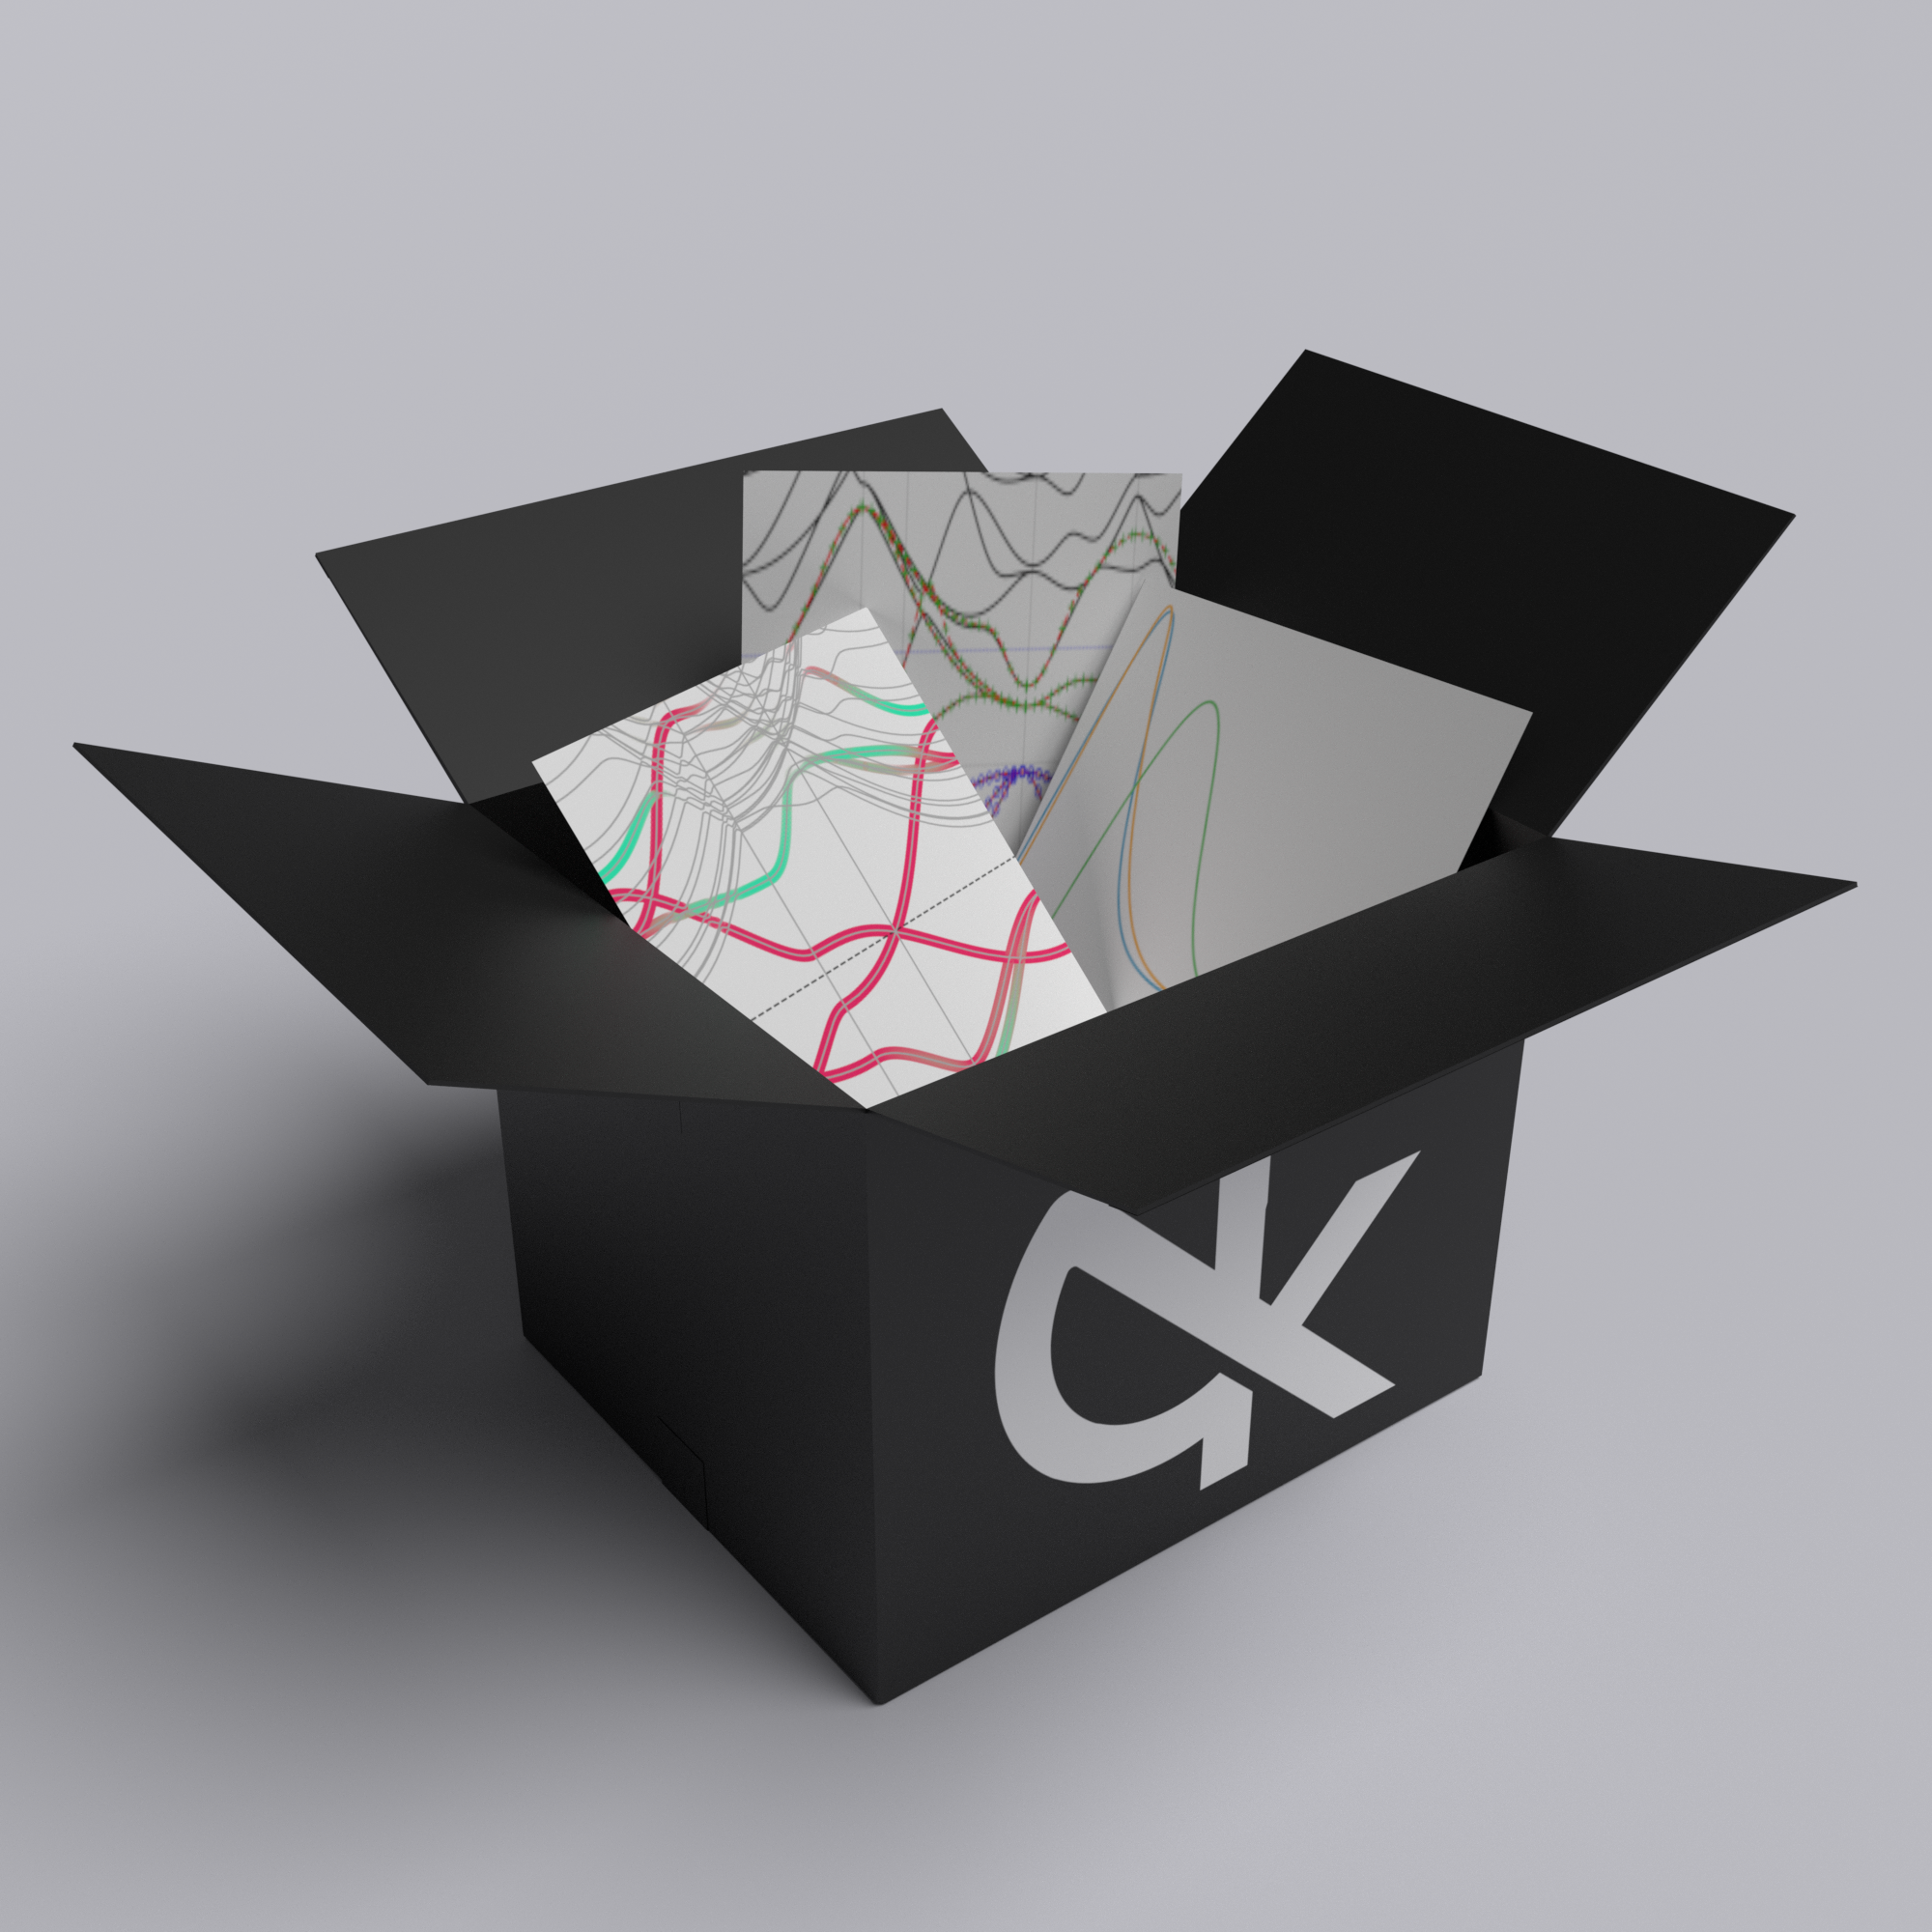
\includegraphics[height=0.99\paperheight]{figures/black_box_filled_square.png}
    \end{column}
    \begin{column}{\dimexpr\paperwidth-0.99\paperheight}
      \vfill
      \bf
      \Large
      \emph{\inserttitle}

      \vspace{0.5em}
      \normalsize
      \insertauthor

      \vspace{0.25em}
      \scriptsize
      \insertinstitute
      
      \vfill
    \end{column}
  \end{columns}
  \vspace{-0.02\paperheight}
  \begin{tcolorbox}[width=0.976\paperwidth, enhanced, colback=kgrey, grow to left by=0.035\paperwidth,]
  %  \begin{center}
  %  \footnotesize\bf\insertauthor\quad \raisebox{0.1ex}{|} \quad \insertshortinstitute\ \quad \raisebox{0.1ex}{|} \quad THEOS Group Meeting \quad \raisebox{0.1ex}{|} \quad \insertdate \quad \raisebox{0.1ex}{|} \quad \includegraphics[height=1.5ex]{logos/SNF_logo_standard_web_sw_neg_e.png} \ \ \includegraphics[height=1.5ex]{logos/logo_marvel_color_transparent_inverted.png}
  %  \end{center}
  \vspace{-0.7ex}
  \hfill \footnotesize\bf\hfill \raisebox{-1.1ex}{\includegraphics[height=3.4ex]{logos/psi_on_transparent.png}} \hfill \raisebox{0.1ex}{|} \hfill DPG conference \hfill \raisebox{0.1ex}{|} \hfill \insertdate \hfill \raisebox{0.1ex}{|} \hfill \includegraphics[height=1.5ex]{logos/SNF_logo_standard_web_sw_neg_e.png} \ \ \includegraphics[height=1.5ex]{logos/logo_marvel_color_transparent_inverted.png} \ \qquad \qquad \hfill
  \end{tcolorbox}
}
%\setbeamerfont{frametitle}{series=\bfseries}
\setbeamertemplate{footline}
{
}

% Title slide %%%%%%%%%%%%%%%%%%%%%%%%%%%%%%%%%%%%%%%%%%%%%%%%%%%%%%%%%%%%%%%%%%%%%%%%%%%%%%%%%%%
\author{Edward Linscott}
\institute{Laboratory for Materials Simulations\\Paul Scherrer Institute}
\date{21 March 2024}
\title{Black-box, accurate, and efficient prediction of band structures with Koopmans functionals}
% \subtitle{or: getting lost down a pseudopotential-generation rabbit hole}
\begin{document}

\definecolor{grey_from_blender}{HTML}{b9b9c0}
\setbeamercolor{background canvas}{bg=grey_from_blender}

\frame{\titlepage}
% \frame{\titlepage}
\setbeamercolor{background canvas}{bg=white}

\begin{frame}{Accurate band structures}
   How can we calculate charged excitations (i.e. band structures, photoemission) accurately and efficiently?

   \vspace{-1ex}

   \begin{columns}
      \begin{column}{0.5\textwidth}
         \begin{description}[<+(1)->]
            \item[DFT] intrinsic failure
            \item[GW] accurate but more expensive; diagrammatic
            \item[Koopmans] accurate band structures with a functional theory
         \end{description}
         \onslide<5->{
            \vspace{1ex}
            \footnotesize
            \begin{tabular}{c S[table-format = 2.2] S[table-format = 2.2] >{\color{seaborn_red}\bfseries}S[table-format = 2.2] >{\color{seaborn_red}\bfseries}S[table-format = 2.2] S[table-format = 2.2]}
                                & {PBE} & {G\textsubscript{0}W\textsubscript{0}} & {KI} & {KIPZ} & {QSG$\tilde{\mathsf{W}}$} \\
               \midrule
               \midrule
               $E_\mathsf{gap}$ & 2.54  & 0.56                                   & 0.27 & 0.22   & 0.18                      \\
               %                                  & {MAPE (\%)} & 48.28 & 12.10      & 7.0           \\
               \midrule
               IP               & 1.09  & 0.39                                   & 0.19 & 0.21   & 0.49                      \\
               %                                  & {MAPE (\%)} & 15.58 & 5.71                                   & 2.99 & 3.14   & 7.41
            \end{tabular}

         }
      \end{column}
      \begin{column}{0.5\textwidth}
         \begin{center}
            \onslide<4->{
               \includegraphics[width=0.8\textwidth]{figures/fig_nguyen_prx_bandgaps.png}
            }
         \end{center}
      \end{column}
   \end{columns}
   \blfootcite{Nguyen2018}

\end{frame}

\begin{frame}{Features of Koopmans functionals}
   \begin{align*}
      E_\mathsf{Koopmans}[\rho,{\{f_i\}}, {\{\alpha_i\}}]
      = {E_{DFT}[\rho]}
      + \sum_i
      {\alpha_i}
      \Biggl(
      -
      {\int^{f_i}_{0} \varepsilon_i(f) df}
      +
      {f_i {\eta_i}}
      \Biggr)
   \end{align*}
   General features:
   \begin{itemize}[<+(1)->]
      \item a correction to DFT that ensures eigenvalues match total energy differences
      \item is orbital-density-dependent (gives rise to, and is reliant on, a localised set of orbitals)
      \item requires screening parameters $\alpha_i$ to be calculated
   \end{itemize}

   \onslide<5->{
      In order to evaluate this functional, one must...
   }
   \begin{enumerate}[<+(2)->]
      \item perform a Wannierisation
      \item calculate the screening parameters $\{\alpha_i\}$
      \item minimize the functional
      \item diagonalize the Hamiltonian
   \end{enumerate}

\end{frame}

\begin{frame}{What needs to be in the box?}

   \begin{columns}
      \begin{column}{0.5\textwidth}
         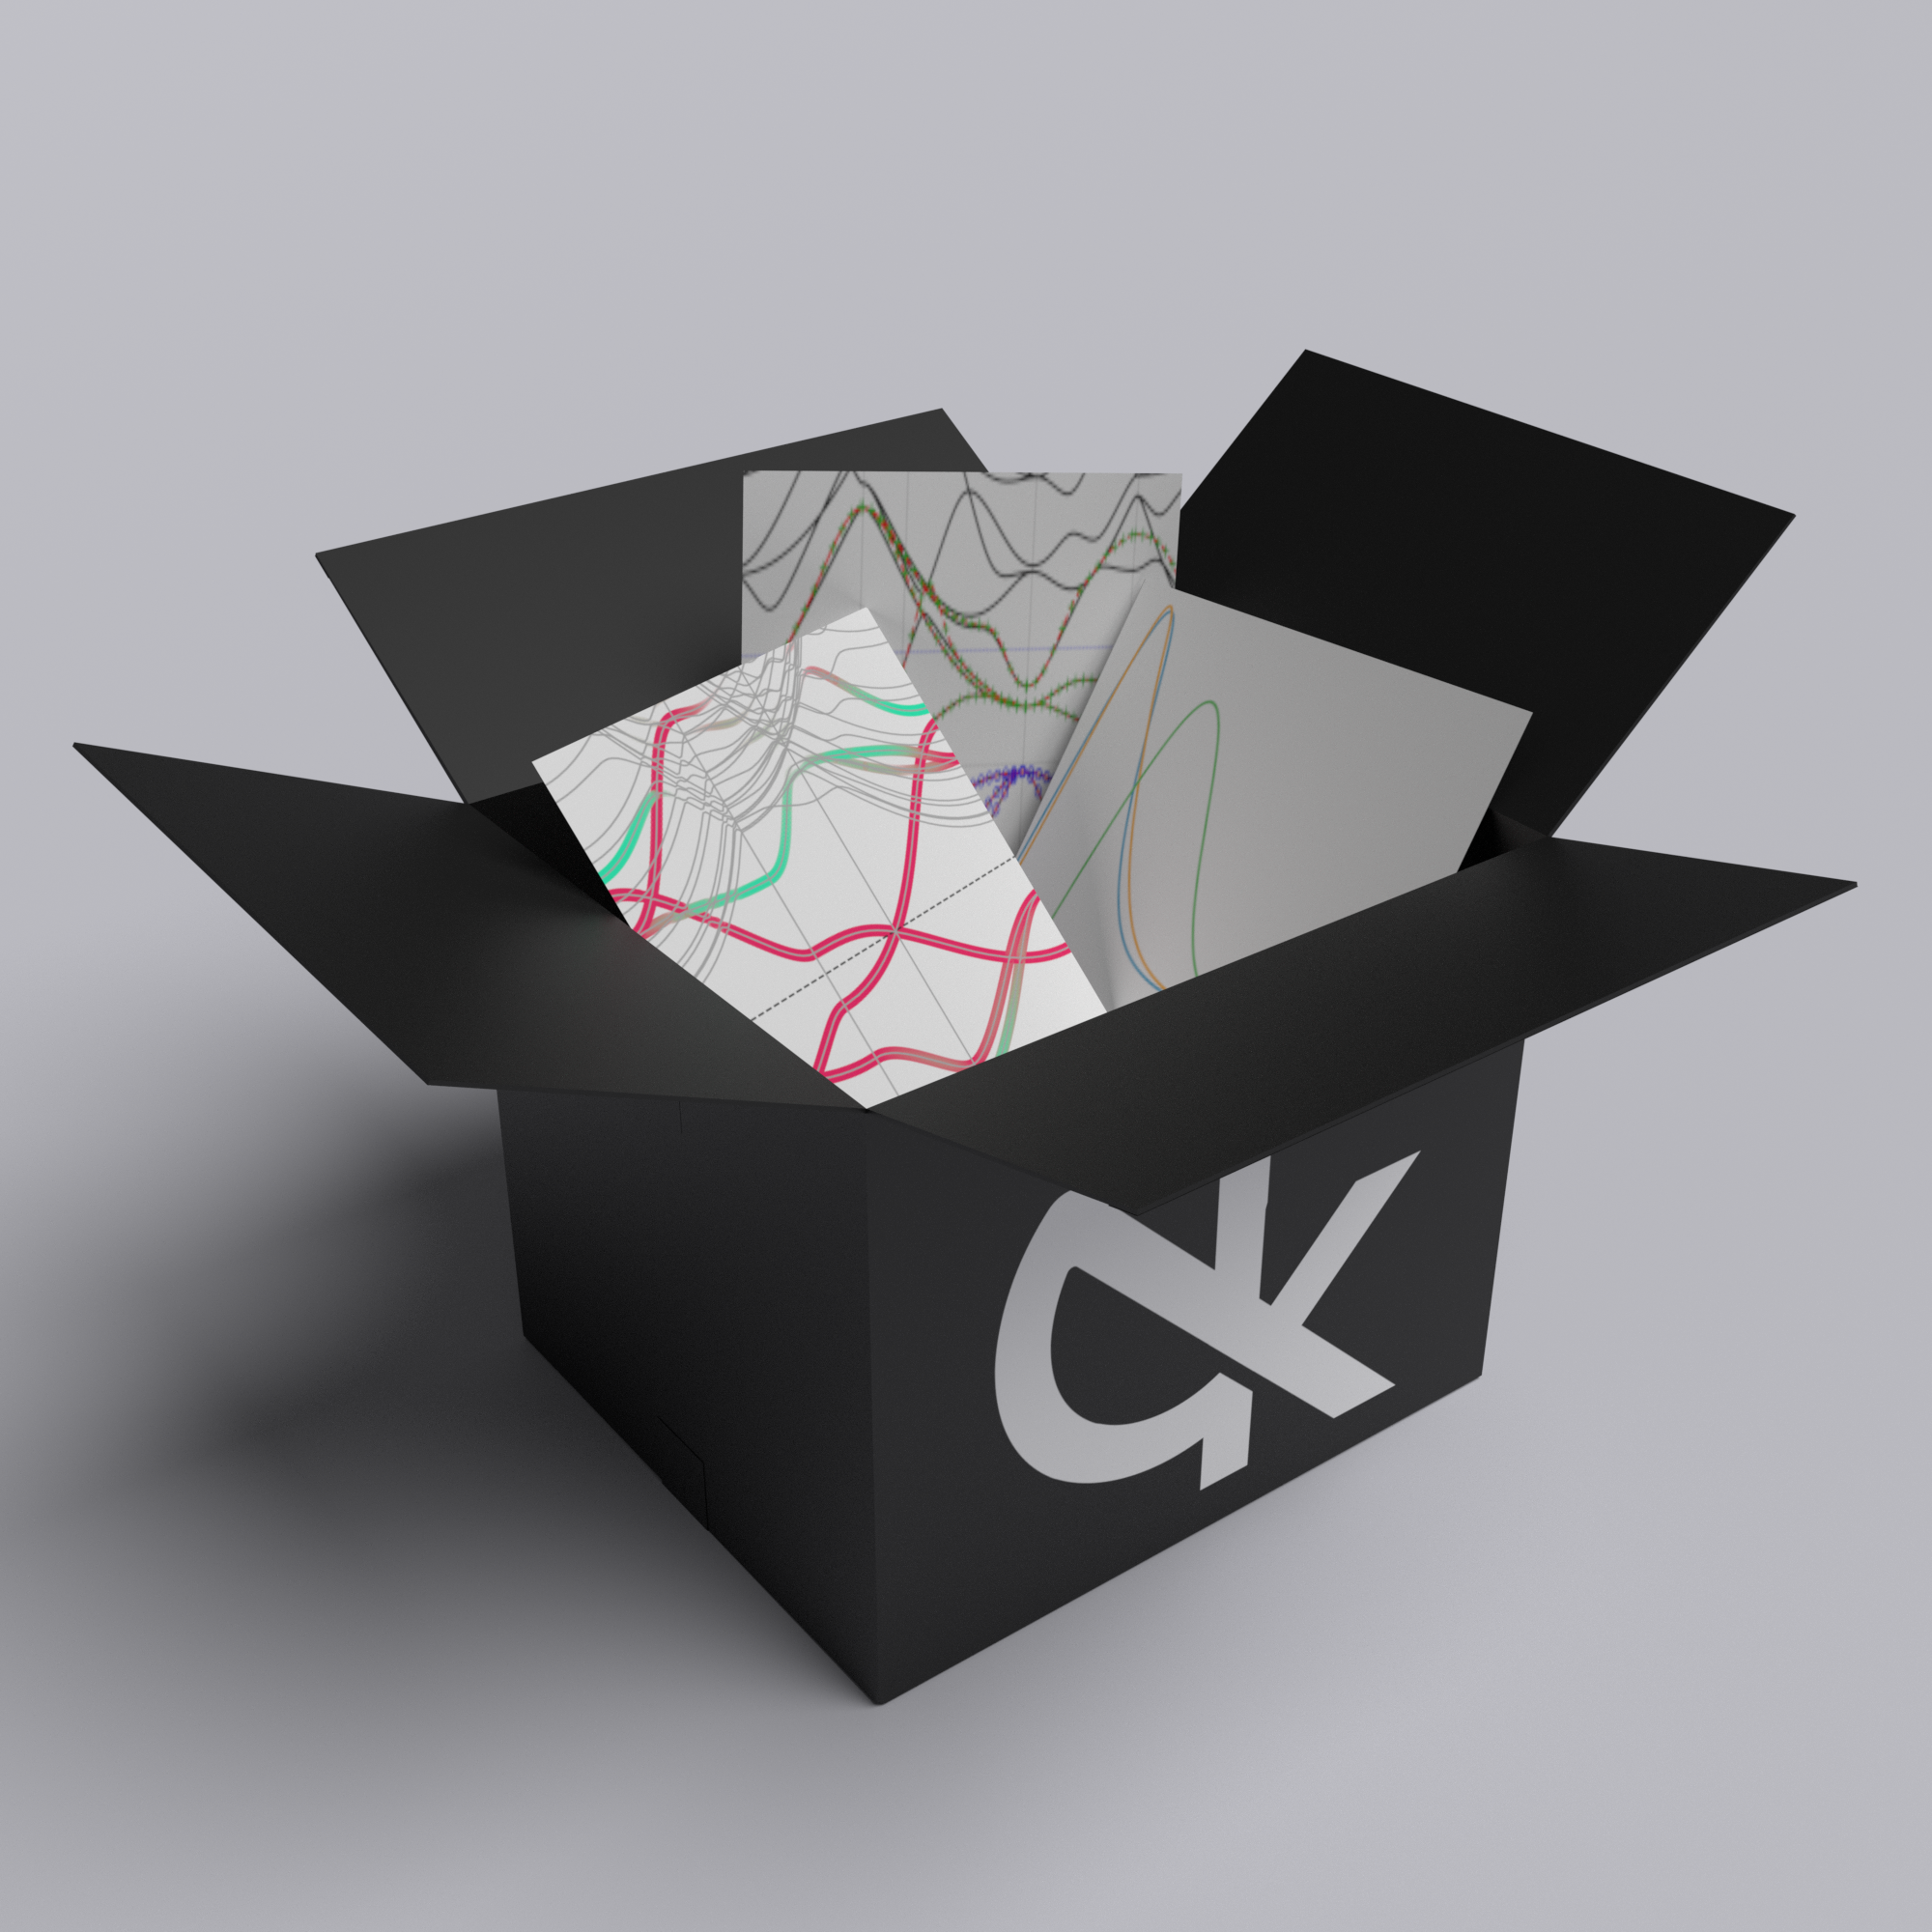
\includegraphics[width=\columnwidth]{figures/black_box_filled_square.png}
      \end{column}
      \begin{column}{0.5\textwidth}
         For a black box, we need...

         \vspace{1ex}
         \onslide<2->{\ $\square$ automated start-to-finish calculations}

         \vspace{1ex}
         \onslide<3->{\ $\square$ minimal input required from the user}
      \end{column}
   \end{columns}
\end{frame}

\begin{frame}{}
   \begin{center}
      \includegraphics[width=0.6\textwidth]{figures/koopmans_grey_on_transparent.png}
   \end{center}

   \vspace{-2ex}

   \begin{columns}
      \begin{column}{0.55\textwidth}
         \begin{itemize}
            \item v1.0 released last year\footnotemark[1]
            \item implementations of Koopmans functionals within Quantum ESPRESSO
            \item automated workflows
                  \begin{itemize}
                     \item Koopmans calculations
                     \item Wannierisation
                     \item dielectric tensor
                     \item ...
                  \end{itemize}
            \item built on top of ASE\footnotemark[2]
            \item does not require expert knowledge
         \end{itemize}
      \end{column}

      \begin{column}{0.4\textwidth}
         \centering
         \url{koopmans-functionals.org}
         \includegraphics[width=\columnwidth]{figures/website_cropped.png}
      \end{column}
   \end{columns}
   \footnotetext[1]{\cite{Linscott2023}}
   \footnotetext[2]{\cite{Larsen2017}}
\end{frame}

\begin{frame}{}
   \includegraphics[width=\textwidth]{figures/jctc.png}
\end{frame}

\begin{frame}{What needs to be in the box?}

   \begin{columns}
      \begin{column}{0.5\textwidth}
         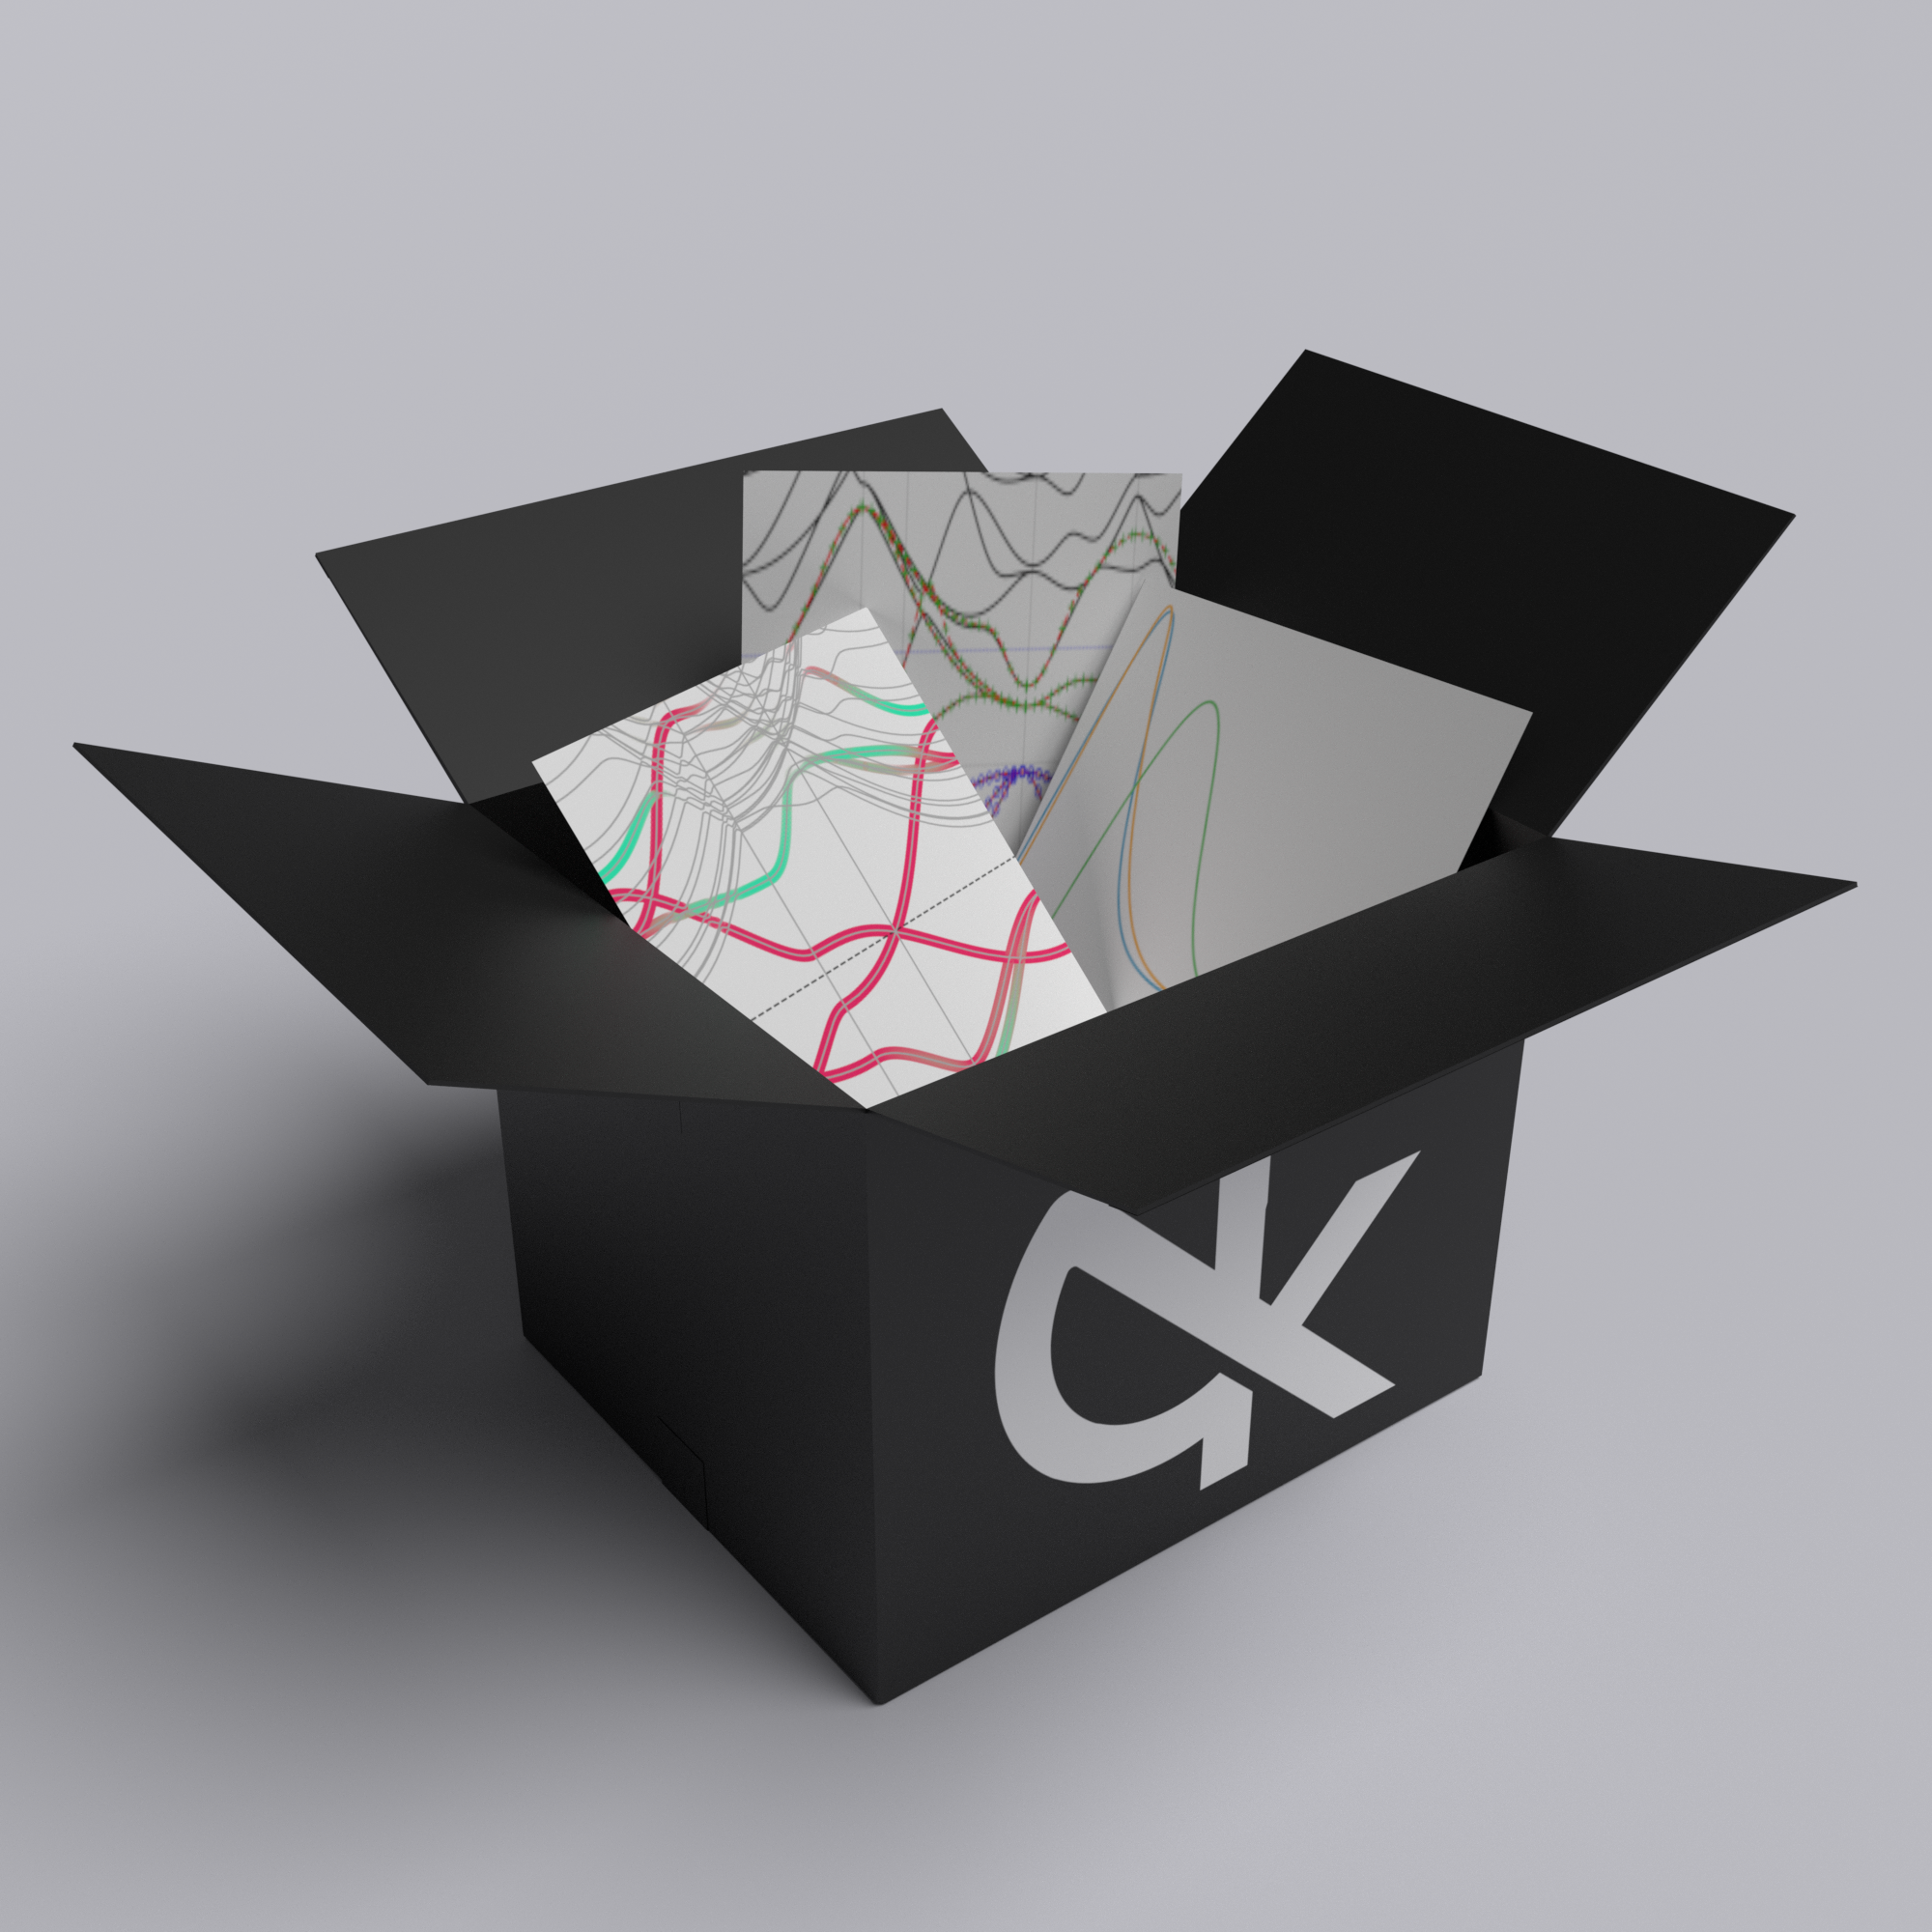
\includegraphics[width=\columnwidth]{figures/black_box_filled_square.png}
      \end{column}
      \begin{column}{0.5\textwidth}
         For a black box, we need...

         \vspace{1ex}
         \
         \only<1>{$\square$}%
         \only<2->{%
            \rlap{$\square$}{\raisebox{2pt}{\large\hspace{1pt}\ding{51}}}%
            \hspace{-1.5pt}}%
         \ automated start-to-finish calculations

         \vspace{1ex}
         \ $\square$ minimal input required from the user
      \end{column}
   \end{columns}
\end{frame}
% 
\begin{frame}{Automating Wannierisation}

   \begin{columns}
      \begin{column}{0.5\textwidth}
         One step still very manual: Wannierisation

         Can we automate it?

         \begin{itemize}[<+(1)->]
            \item use PAOs found in pseudopotential files as initial guesses for Wannier functions
            \item projectability-based disentanglement instead of energy-based disentanglement
            \item use a parallel transport algorithm to separate the occupied and empty manifolds
         \end{itemize}
      \end{column}
      \begin{column}{0.5\textwidth}
         \begin{overlayarea}{\columnwidth}{0.6\paperheight}
            \begin{center}
               \only<2>{\includegraphics[width=0.8\columnwidth]{figures/plot_paos/old_projs.png}}
               \only<3>{\includegraphics[height=0.6\paperheight]{figures/proj_disentanglement_fig1a.png}}
               \only<4>{\includegraphics[width=\columnwidth]{figures/target_manifolds_fig1b.png}}
            \end{center}
         \end{overlayarea}
      \end{column}
   \end{columns}
   % \begin{figure}[t]
   %    \begin{subfigure}{0.2\textwidth}
   %       \onslide<2->{
   %       \includegraphics[height=1.5\columnwidth]{figures/proj_disentanglement_fig1b.png}
   %       \vspace{-0.01\paperheight}
   %       }
   %    \end{subfigure}
   %    \begin{subfigure}{0.2\textwidth}
   %       \onslide<3->{
   %       \includegraphics[height=1.5\columnwidth]{figures/proj_disentanglement_fig1a.png}
   %       }
   %    \end{subfigure}
   %    \hspace{0.025\textwidth}
   %    % \begin{subfigure}{0.225\textwidth}
   %    %    \onslide<3->{
   %    %    \includegraphics[height=1.5\columnwidth]{figures/proj_disentanglement_fig1d.png}
   %    %    }
   %    % \end{subfigure}
   %    \begin{subfigure}{0.2\textwidth}
   %       \onslide<4->{
   %       \includegraphics[height=1.5\columnwidth]{figures/proj_disentanglement_fig1f.png}
   %       }
   %    \end{subfigure}
   % \end{figure}

   \blfootcite{Agapito2013}
   \blfootcite{Qiao2023,Qiao2023a}

\end{frame}

\begin{frame}{Automating Wannierisation}
   \vspace{-2ex}
   \begin{columns}
      \begin{column}{0.5\textwidth}
         \includegraphics[width=\columnwidth]{figures/TiO2_wannierize_bandstructure.png}
      \end{column}
      \begin{column}{0.5\textwidth}
         \onslide<2->{
            \inputminted[fontsize=\tiny]{json}{scripts/TiO2.json}
         }
      \end{column}
      % \hbox{
      %    \raisebox{0.15\textwidth}{\huge $\rightarrow$}
      % }
   \end{columns}
\end{frame}

\begin{frame}{Automating Wannierisation}

   A drawback: the number of Wannier functions is determined by the number of PAOs in the pseudopotentials\onslide<2->{... which can be a problem e.g. LiF}

   \begin{columns}
      \begin{column}{0.5\textwidth}
         \onslide<3->{

            \begin{center}
               \footnotesize
               \begin{tabular}[h]{ccc}
                  element & configuration                                                                                             & {PAOs}                                                              \\
                  \hline
                  Li      & 1s\textsuperscript{2} 2s\textsuperscript{1}                                                               & {1s, 2s}                                                            \\
                  {F}     & {\textcolor{seaborn_bg_grey_darker}{[1s\textsuperscript{2}]} 2s\textsuperscript{2} 2p\textsuperscript{5}} & {2s, 2p\textsubscript{x}, 2p\textsubscript{y}, 2p\textsubscript{z}} \\
               \end{tabular}
            \end{center}
         }
         \vspace{1ex}
         \onslide<5->{If we want a better representation of the conduction bands, we're gonna need \sout{a bigger boat} more PAOs...}
      \end{column}
      \begin{column}{0.5\textwidth}
         \vspace{1ex}
         \onslide<4->{\includegraphics[width=\textwidth]{figures/LiF_bandstructures/default.png}}

      \end{column}

   \end{columns}

\end{frame}

\begin{frame}{Automating Wannierisation}

   \vspace{-2ex}
   \begin{center}
      \includegraphics[width=0.3\textwidth]{figures/plot_paos/old_projs.png}
      \raisebox{0.15\textwidth}{\huge $\rightarrow$}
      \includegraphics[width=0.3\textwidth]{figures/plot_paos/new_projs.png}
   \end{center}

   \vspace{-2ex}
   For cases such as LiF:

   \begin{itemize}[<+->]
      \item re-solve the radial Schrödinger equation for higher subshells
      \item apply a confining potential while doing so
      \item optimize the confining potential to maximise projectability
      \item N.B. only once per pseudopotential
   \end{itemize}


\end{frame}

\begin{frame}{Automating Wannierisation}
   \begin{center}
      \hbox{
         \includegraphics[width=0.45\textwidth]{figures/LiF_bandstructures/default.png}
         \onslide<2->{
         \raisebox{0.15\textwidth}{\huge $\rightarrow$}
         \includegraphics[width=0.45\textwidth]{figures/LiF_bandstructures/Li_only.png}
         }
      }

      \onslide<3->{
      \begin{tabular}{c *{6}{d{2.2}}}
         & \multicolumn{1}{c}{LDA}
         & \multicolumn{1}{c}{HSE}
         & \multicolumn{1}{c}{GW\textsubscript{0}}
         & \multicolumn{1}{c}{scG$\tilde{\mathsf{W}}$}
         & \multicolumn{1}{c}{KI}
         & \multicolumn{1}{c}{exp} \\
         \hline
         $E_\mathsf{gap}$ (eV) & 8.87 & 11.61 & 13.96 & 14.5 & 15.28 & 15.35
      \end{tabular}
      \blfootcite{Colonna2022}
      }
   \end{center}


\end{frame}
% 
% \begin{frame}{Next steps...}
%    \begin{itemize}[<+(1)->]
%       \item decide on a criteria for choosing the confining potential parameters (depth, width, and smoothness)
%       \item if the parameters are system-independent, publish a periodic table of PAOs
%       \item tidy and publish modified \texttt{oncvpsp.x}
%       \item finally do some Koopmans calculations! (Would need a good criteria for which elements to extend)
%    \end{itemize}
% 
%    \onslide<6->{Nice to have but not essential:}
%    \begin{itemize}[<+(2)->]
%       \item investigate/resolve bad Wannier90 convergence
%       \item the option to use external projectors in \texttt{projwfc.x}
%    \end{itemize}
% 
% \end{frame}
% 
% \begin{frame}{\footnotesize Maybe the real treasure is the python packages we made along the way}
% 
%    \hbox{
%       \includegraphics[width=0.5\textwidth]{figures/upf-tools.png}
%       \includegraphics[width=0.5\textwidth]{figures/oncvpsp-tools.png}
%    }
% \end{frame}
% 
% \begin{frame}{\footnotesize Maybe the real treasure is the python packages we made along the way}
% 
%    Publish your code!
%    \begin{itemize}
%       \item It's easy: most of the infrastructure was from the \texttt{cookiecutter} I used (see my July 2022 GM)
%       \item It avoids duplication: \texttt{upf-tools} was discovered by Marnik and is now used in \texttt{AiiDA}
%    \end{itemize}
% 
% \end{frame}
\begin{frame}{Take home messsages}

   \begin{columns}
      \begin{column}{0.5\textwidth}
         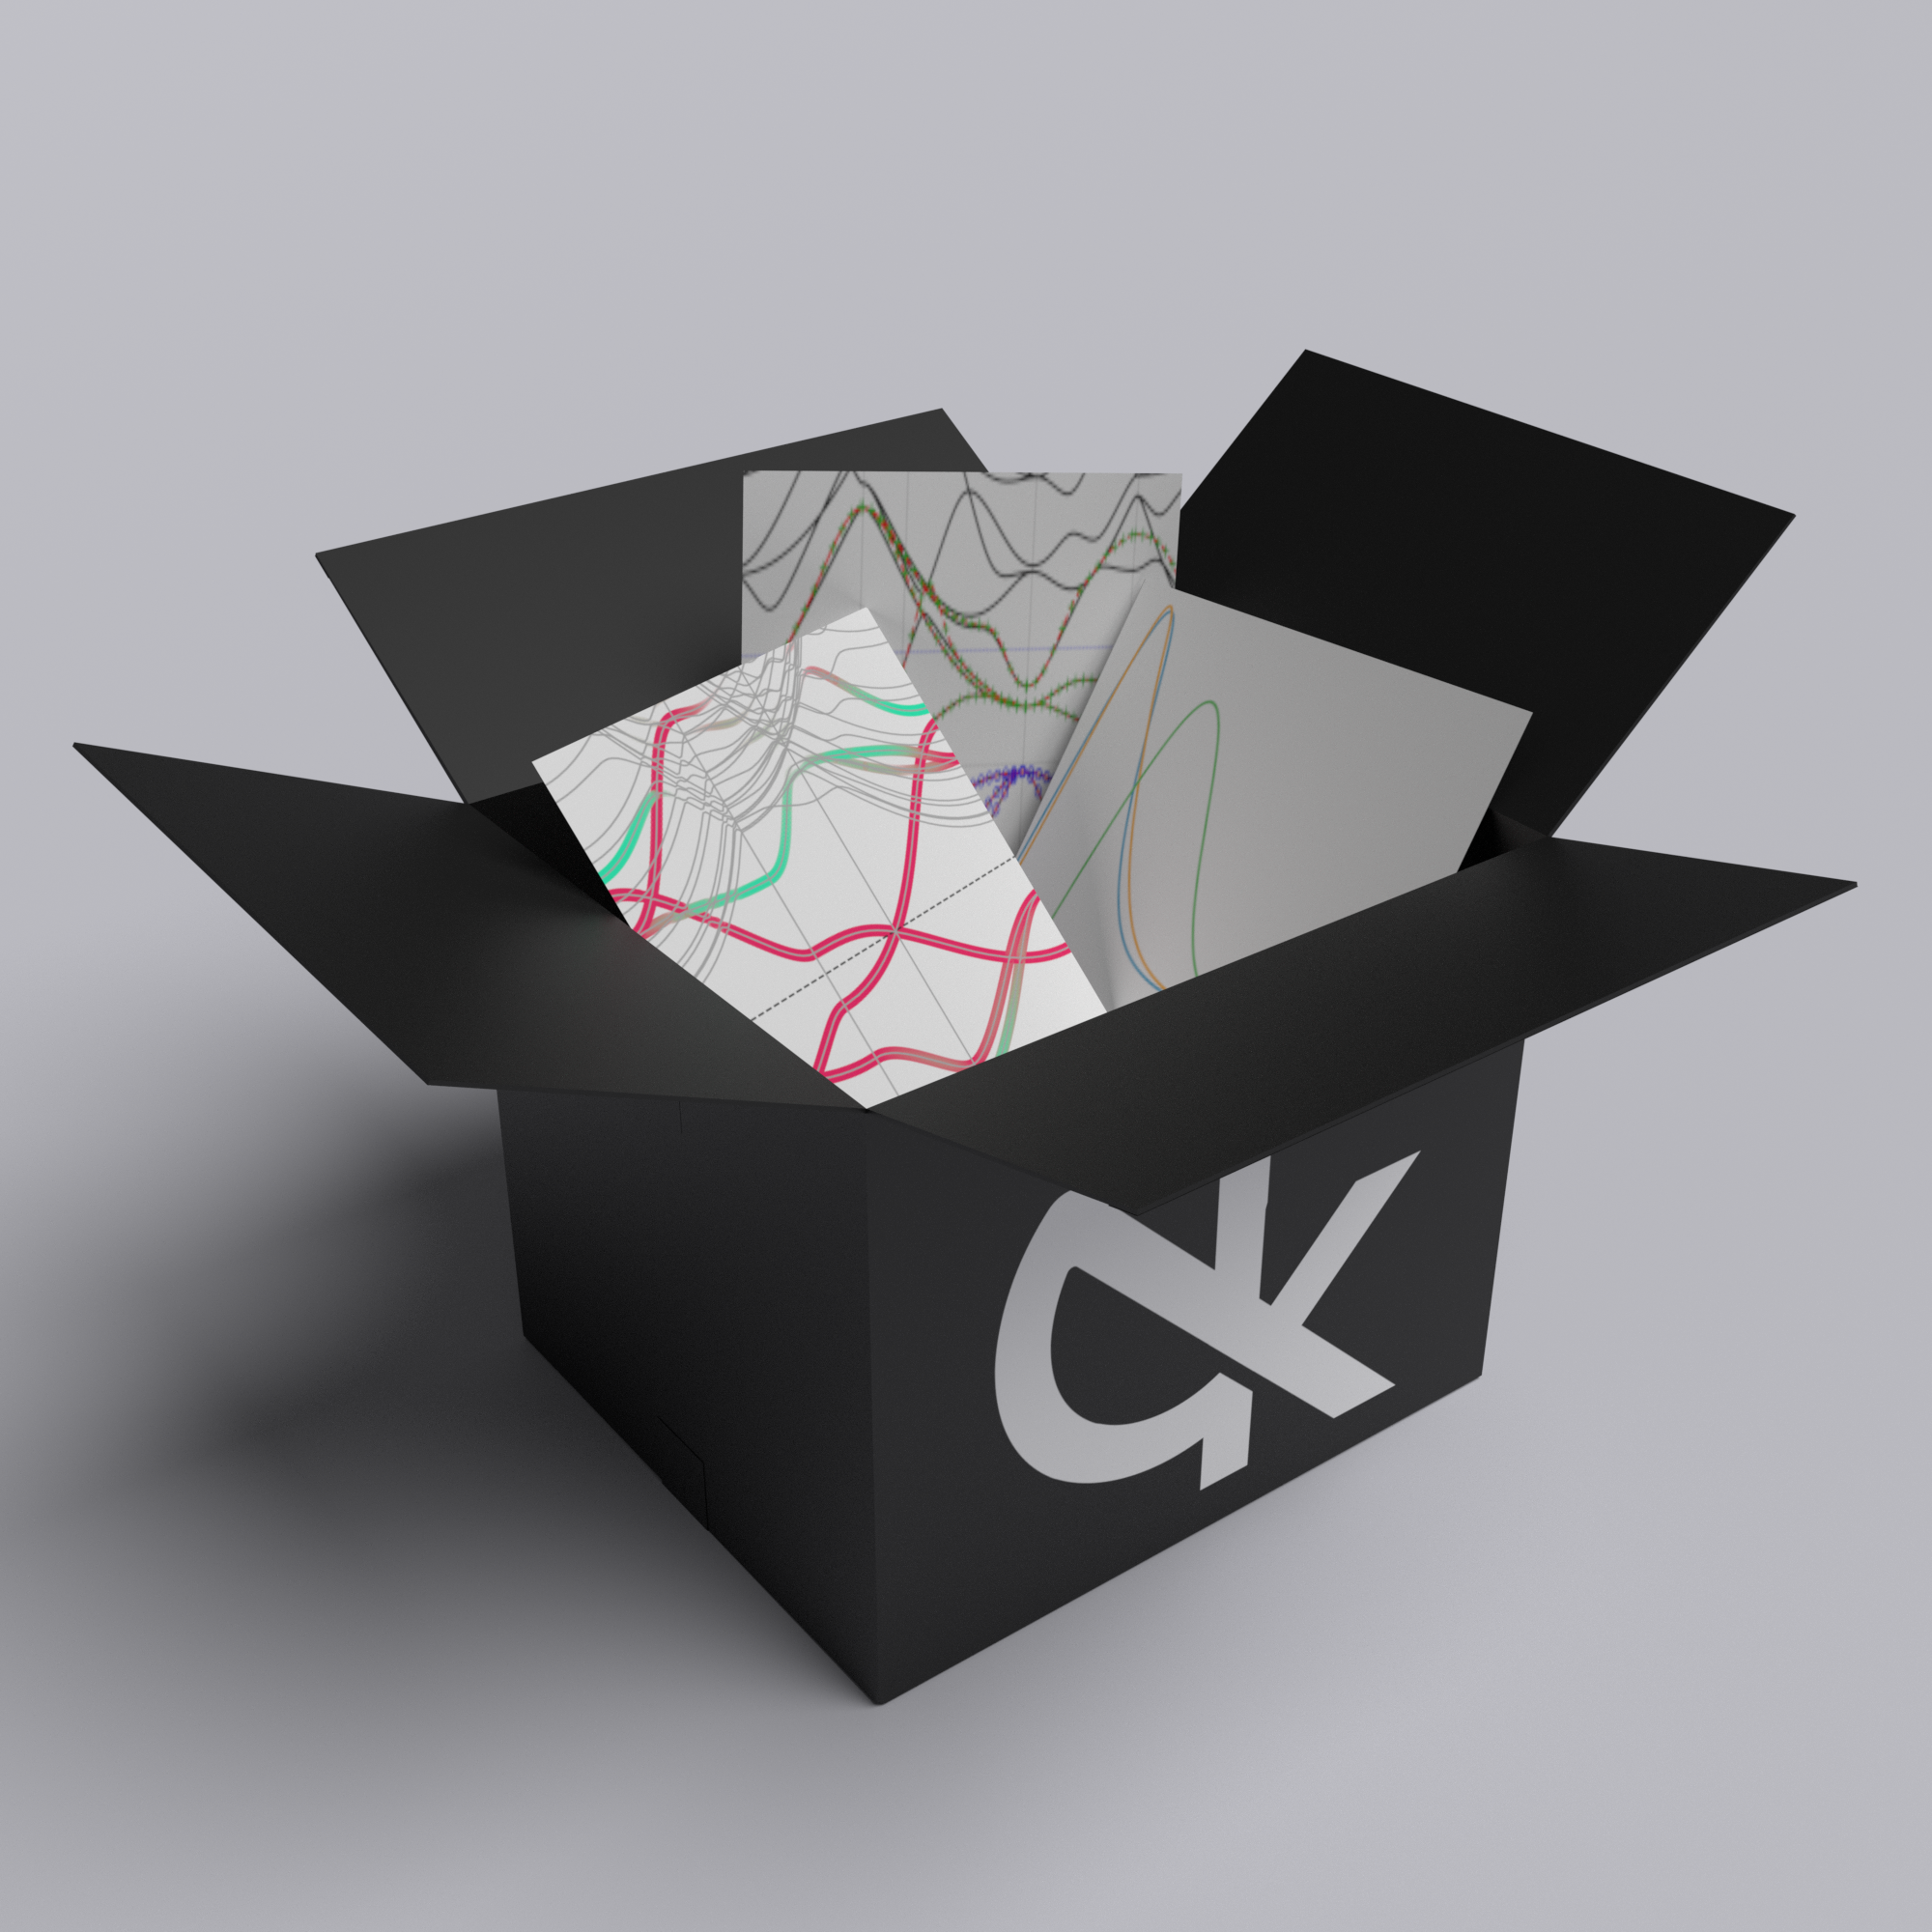
\includegraphics[width=\columnwidth]{figures/black_box_filled_square.png}
      \end{column}
      \begin{column}{0.5\textwidth}

         Koopmans functionals can accurately and efficiently predict the band structure of materials

         \vspace{1ex}
         To make these calculations black box, we have...

         \vspace{1ex}
         \ \only<1>{$\square$}%
         \only<2->{%
            \rlap{$\square$}{\raisebox{2pt}{\large\hspace{1pt}\ding{51}}}%
            \hspace{-1.5pt}}%
         \ automated start-to-finish calculations \onslide<2->{\emph{with the \texttt{koopmans} package}}

         \vspace{1ex}
         \ \only<1-2>{$\square$}%
         \only<3->{%
            \rlap{$\square$}{\raisebox{2pt}{\large\hspace{1pt}\ding{51}}}%
            \hspace{-1.5pt}}%
         \ minimal input required from the user \onslide<3>{\emph{enabled via automated Wannierisation}}
      \end{column}
   \end{columns}
\end{frame}

\begingroup
\setbeamertemplate{footline}{}
\begin{frame}{Acknowledgements}
   \begin{center}
      \footnotesize
      \begin{tabularx}{0.7\textwidth}{CCC}
         \includegraphics[height = 0.3\paperheight]{figures/nicola_marzari.jpg}  &
         \includegraphics[height = 0.3\paperheight]{figures/nicola_colonna2.png} &
         \includegraphics[height = 0.3\paperheight]{photos/junfeng.jpeg}           \\
         % \includegraphics[height = 0.2\paperheight]{figures/daniel_cole.jpeg}       &
         % \includegraphics[height = 0.2\paperheight]{figures/mike_payne.jpeg}        &
         % \includegraphics[height = 0.2\paperheight]{figures/david_oregan.jpg}         \\
         Nicola Marzari                                                          &
         Nicola Colonna                                                          &
         Junfeng Qiao
      \end{tabularx}
   \end{center}

   \vspace{2ex}

   \begin{center}
      \includegraphics[height = 0.15\paperheight]{logos/SNF_logo_standard_print_color_pos_e.eps}
      \hspace{3em}
      \includegraphics[height = 0.15\paperheight]{figures/marvel_trimmed.png}
   \end{center}

   \vspace{1ex}

   \begin{center}
      Want to find out more? Go to \url{koopmans-functionals.org}

      \vspace{1em}
      Follow \includegraphics[height=\fontcharht\font`\B]{figures/Twitter_Bird.png} \textcolor{twitter_blue}{@ed\_linscott} for updates | Slides available at \includegraphics[height=\fontcharht\font`\B]{logos/github-favicon.png} github/elinscott
   \end{center}

   % \begin{multicols}{2}
   %    \tiny
   %    \printbibliography
   %    \normalsize
   % \end{multicols}
   \vspace{2ex}
   \scriptsize

   \setbeamercolor*{bibliography entry title}{fg=black}
   \setbeamercolor*{bibliography entry author}{fg=black}
   \setbeamercolor*{bibliography entry location}{fg=black}
   \setbeamercolor*{bibliography entry note}{fg=black}

   \vspace{2ex}
   \scriptsize
\end{frame}
\endgroup
\backupbegin
\begin{frame}{}

   \begin{center}
      \huge SPARE SLIDES
   \end{center}

\end{frame}

\begin{frame}{Localised states}
   Consequences of ODD:
   \begin{itemize}[<+(1)->]
      \item variational (localized, minimizing) vs canonical (delocalized, diagonalizing) orbitals
            \begin{figure}[t]
               \centering
               \begin{subfigure}{0.3\textwidth}
                  \includegraphics[height=\columnwidth,angle=90]{figures/fig_nguyen_variational_orbital.png}
                  \caption{variational}
               \end{subfigure}
               \hspace{0.1\textwidth}
               \begin{subfigure}{0.3\textwidth}
                  \includegraphics[height=\columnwidth,angle=90]{figures/fig_nguyen_canonical_orbital.png}
                  \caption{canonical}
               \end{subfigure}
            \end{figure}
      \item Practically we can often use MLWFs
      \item localized variational orbitals naturally allow us to treat bulk systems
      % \item ODD functional means that we know $\hat H \ket{\varphi_i}$ for variational orbitals $\{\ket{\varphi_i}\}$ but we don't know $\hat H$ in general
   \end{itemize}
   \blfootcite{Nguyen2018}
\end{frame}

\begin{frame}{Localised states}

   \begin{center}
      \includegraphics[width=0.8\textwidth]{figures/fig_nguyen_scaling.png}
   \end{center}
   \onslide<2->{
      \noindent In the bulk limit for one cell $\Delta E_\text{one cell} = E(N-\delta N) - E(N)$
   }%

   \onslide<3>{ 
      Across all the cells $
         \Delta E_\text{all cells} = \frac{1}{\delta N}\left(E(N-\delta N) - E(N)\right) = -\frac{dE}{dN} = -\varepsilon_\mathsf{HO}$
   }%

   \blfootcite{Nguyen2018}

\end{frame}

\begin{frame}{Workflows}
   \onslide<2->{
      (a) finite difference calculations using a supercell

      \vspace{-2ex}
      \adjustbox{width=\textwidth}{\input{supercell_workflow.tex}\end{tikzpicture}}
   }

   \vspace{-1.5ex}
   \onslide<3->{
      (b) DFPT using a primitive cell

      \vspace{-2ex}
      \adjustbox{width=0.655\textwidth}{\input{primitive_workflow.tex}}
   }

   \vspace{2ex}
   \onslide<4->{All implemented in \raisebox{-0.65ex}{\includegraphics[height=2.5ex]{figures/koopmans_grey_on_transparent.png}}}

   \blfootcite{Linscott2023}

\end{frame}

% \begin{frame}{Workflows}
% 
%    What still stands in our way? Take the example of silicon:
% 
%    \onslide<2->{
%       \vspace{-1ex}
%       \inputminted[fontsize=\scriptsize]{json}{scripts/si.json}
%    }
% 
% \end{frame}


\begin{frame}{Accurate band structures}

   \begin{table}[t]
      \centering
      \scriptsize
      \begin{tabular}{r@{ $\rightarrow$ } l *{3}{d{2.2}} >{\color{seaborn_red}}S[table-format = 2.2] >{\color{seaborn_red}}S[table-format = 2.2] d{2.2} @{$\pm$} d{1.2}}
         \hline
         \hline
         \multicolumn{2}{c}{ }
                                   & \multicolumn{1}{c}{PBE}
                                   & \multicolumn{1}{c}{G\textsubscript{0}W\textsubscript{0}\footnote{\cite{Shishkin2007} for $E_g$ and \cite{Hybertsen1986} for the transitions;}}
                                   & \multicolumn{1}{c}{scG$\tilde{\mathsf{W}}$\footcite{Shishkin2007a}}
                                   & \multicolumn{1}{c}{
            \textcolor{seaborn_red}{\bfseries KI@[PBE,MLWFs]}}
                                   & \multicolumn{1}{c}{
            \textcolor{seaborn_red}{\bfseries KIPZ@PBE}}
                                   & \multicolumn{2}{c}{exp\footcite{Madelung2004}}                                                                                                                                                                                             \\
         \hline
         \multicolumn{2}{c}{$E_g$} &
         0.49                      & 1.06                                                                                                                                           & 1.14  & 1.16  & 1.15 & \multicolumn{2}{c}{1.17}                                           \\
         $\Gamma_{1v}$             & $\Gamma_{25'v}$                                                                                                                                & 11.97 & 12.04 &      & 11.97                    & 12.09 & 12.5                     & 0.6  \\
         $X_{1v}$                  & $\Gamma_{25'v}$                                                                                                                                & 7.82  &       &      & 7.82                     &       & \multicolumn{2}{c}{7.75}        \\
         $X_{4v}$                  & $\Gamma_{25'v}$                                                                                                                                & 2.85  & 2.99  &      & 2.85                     & 2.86  & \multicolumn{2}{c}{2.90}        \\
         $L_{2'v}$                 & $\Gamma_{25'v}$                                                                                                                                & 9.63  & 9.79  &      & 9.63                     & 9.74  & 9.3                      & 0.4  \\
         $L_{1v}$                  & $\Gamma_{25'v}$                                                                                                                                & 6.98  & 7.18  &      & 6.98                     & 7.04  & 6.8                      & 0.2  \\
         $L_{3'v}$                 & $\Gamma_{25'v}$                                                                                                                                & 1.19  & 1.27  &      & 1.19                     &       & 1.2                      & 0.2  \\
         $\Gamma_{25'v}$           & $\Gamma_{15c}$                                                                                                                                 & 2.48  & 3.29  &      & 3.17                     & 3.20  & 3.35                     & 0.01 \\
         $\Gamma_{25'v}$           & $\Gamma_{2'c}$                                                                                                                                 & 3.28  & 4.02  &      & 3.95                     & 3.95  & 4.15                     & 0.05 \\
         $\Gamma_{25'v}$           & $X_{1c}$                                                                                                                                       & 0.62  & 1.38  &      & 1.28                     & 1.31  & \multicolumn{2}{c}{1.13}        \\
         $\Gamma_{25'v}$           & $L_{1c}$                                                                                                                                       & 1.45  & 2.21  &      & 2.12                     & 2.13  & 2.04                     & 0.06 \\
         $\Gamma_{25'v}$           & $L_{3c}$                                                                                                                                       & 3.24  & 4.18  &      & 3.91                     & 3.94  & 3.9                      & 0.1  \\
         \hline
         \multicolumn{2}{c}{MSE}   & 0.35                                                                                                                                           & 0.02  &       & 0.01 & 0.03                                                               \\
         \multicolumn{2}{c}{MAE}   & 0.44                                                                                                                                           & 0.21  &       & 0.14 & 0.17                                                               \\
         \hline
         \hline
      \end{tabular}

      % \textsuperscript{\emph{a}} this work;
      % \textsuperscript{\emph{b}} Ref.~\citenum{Shishkin2007} for $E_g$ and Ref.~\citenum{Hybertsen1986} for the transitions;
      % \textsuperscript{\emph{c}} Ref.~\citenum{Shishkin2007a};
      % \textsuperscript{\emph{d}} Ref.~\citenum{DeGennaro2022};
      % \textsuperscript{\emph{e}} Ref.~\citenum{Madelung2004}
   \end{table}
\end{frame}
% 
% \begin{frame}{Spare slide}
% \end{frame}
% 
% 
\begin{frame}{\normalsize Koopmans functionals give accurate band structures}
   \begin{figure}[t]
      \centering
      \begin{subfigure}{0.25\textwidth}
         \includegraphics[width=\columnwidth]{figures/ZnO_lda.png}
      \end{subfigure}
      \begin{subfigure}{0.25\textwidth}
         \includegraphics[width=\columnwidth]{figures/ZnO_hse.png}
      \end{subfigure}
      \begin{subfigure}{0.25\textwidth}
         \includegraphics[width=\columnwidth]{figures/ZnO_ki.png}
      \end{subfigure}
      \begin{subfigure}{\textwidth} %<-- changed width
         \centering
         %    \renewcommand\tabularxcolumn[1]{m{#1}}% <-- added
         %    \renewcommand\arraystretch{1.3}
         %    \setlength\tabcolsep{2pt}% <-- added
         \begin{tabular}{c S[table-format = 2.2] S[table-format = 2.2] S[table-format = 2.2] S[table-format = 2.2] >{\color{seaborn_red}\bfseries}S[table-format = 2.2] S[table-format = 2.2]}
            ZnO                                  & {LDA} & {HSE} & {GW$_0$} & {scG$\tilde{\sf W}$} & {KI} & {exp}       \\
            \hline
            $E_\mathsf{gap}$ (eV)                & 0.79  & 2.79  & 3.0      & 3.2                  & 3.62 & 3.60        \\
            $\langle \varepsilon_d \rangle$ (eV) & -5.1  & -6.1  & -6.4     & -6.7                 & -6.9 & {-7.5/-8.0} \\
         \end{tabular}
         %        \caption{table}
      \end{subfigure}
      % \caption{Band structure of ZnO calculated at different level of theory:
      %    LDA (left panel), HSE (middle panel) and KI (right panel). Shaded areas
      %    highlight valence (light blue) and conduction (light red) manifolds. The
      %    experimental values for the band gap and for the energy position of
      %    Zn $d$-states are represented by the dashed green line and by the dashed
      %    red line, respectively.
      %    Table: Band gap and position of Zn $d$ states with respect to the top of the valence band at different level of theory compared to experimental and GW results from Ref.~\onlinecite{shishkin_accurate_2007}.}
   \end{figure}
   \blfootcite{Colonna2022}
\end{frame}

\begin{frame}{Koopmans functionals: results for molecules}
   \small
   Ionisation potentials $ = E(N-1) - E(N) \stackrel{?}{=} -\varepsilon_{HO}$ of 100 molecules (the GW100 set) cf. CCSD(T)
   \begin{center}
      \includegraphics[height=0.2\textwidth]{figures/colonna_2019_gw100_ip}
      % \onslide<2->{\includegraphics[height=0.23\textwidth]{figures/colonna_2019_gw100_deeper}}
   \end{center}

   \vspace{-3ex}
   Ultraviolet photoemission spectra
   \begin{center}
      \begin{tikzpicture}
         \node [inner sep=0pt](fig) at (0,0) {\includegraphics[height=0.35\textheight]{figures/fig_nguyen_prl_spectra.png}};
         \draw [very thick, color=seaborn_red] (-5.35,-0.07) rectangle (5.4,1.6);
      \end{tikzpicture}
   \end{center}
   \vspace{-2ex}

   \blfootcite{Colonna2018,Nguyen2015}
\end{frame}

\begin{frame}{Koopmans functionals: results for toy systems}
   For Hooke's atom (two electrons in a harmonic confining potential with Coulombic repulsion)

   \begin{figure}[t]
      \begin{subfigure}{0.4\textwidth}
         \includegraphics[width=\columnwidth]{figures/schubert_vxc.jpeg}
      \end{subfigure}
      \begin{subfigure}{0.4\textwidth}
         \onslide<2->{
            \includegraphics[width=\columnwidth]{figures/schubert_vxc_integrated.jpeg}
         }
      \end{subfigure}
   \end{figure}

   \blfootcite{Schubert2023}
\end{frame}

\begin{frame}{Criteria for ideal projectors}

   The projectability is
   \begin{equation*}
      p_{m\mathbf{k}} = \sum_n |\langle \varphi_n \mid \psi_{m\mathbf{k}}\rangle |^2
   \end{equation*}

   We want a set of projectors such that\dots
   \begin{itemize}
      \item they should have a large overlap with some Kohn-Sham states and a small overlap with all the others% i.e. $p_{m\mathbf{k}}$ should be close to 0 or 1 for all $m$ and $\mathbf{k}$
      \item they should lie within the span of the Kohn-Sham states% i.e. $\sum_{m\mathbf{k}} p_{m\mathbf{k}}$ should be as large as possible
   \end{itemize}

   We can meet these criteria if we maximise the functional
   \begin{equation*}
      F[\{\varphi_n\}] = \frac{1}{N_\mathbf{k} N_w} \sum_{\mathbf{k}} \sum_{m \in \mathcal{S}_\mathbf{k}} p_{m\mathbf{k}}
   \end{equation*}

   where $\mathcal{S}_\mathbf{k}$ corresponds to the $N_w$-largest values of $p_{m\mathbf{k}}$.

\end{frame}

\begin{frame}{Bayesian optimisation}
   \begin{center}
      \includegraphics[height=0.7\paperheight]{figures/Li_bayesian_opt.png}
   \end{center}
\end{frame}

\backupend
\end{document}
